\section{High level components and their interaction}
\label{sec:high-level}

The main high level components of the system are the following:
\begin{description}
	\item[Application server]: this layer contains all the application logic of the system. All the policies, the algorithms and the computation are performed here. This layer offers a service-oriented interface.
	\item[Web server]: this presentation layer provides a web interface to access to the system via web browsers. This layer doesn't contain any application logic.
	\item[Mobile application]: this presentation layer represents the mobile client. It communicates directly with the application server.
	\item[Database]: the data layer is responsible for the data storage and retrieval. It doesn't implement application logic. This layer must guarantee ACID properties.
	\item[Server side plug-ins]: these are the plug-ins which can be used to extend the application server layer:
		\begin{itemize}
		\item ride sharing
		\item ride reservation
		\end{itemize}
	\item[User's browser]: this presentation layer represents the user's browser; it's not under the control of the system and it accesses the web server.
\end{description}

The main components are structured into four layers presented in figure \ref{fig:layers}.

This design choice makes it possible to deploy the application server and the web server on different tiers. It also improves scalability, since there may be many web servers talking to a single application server.

\begin{figure}[h]
\centering
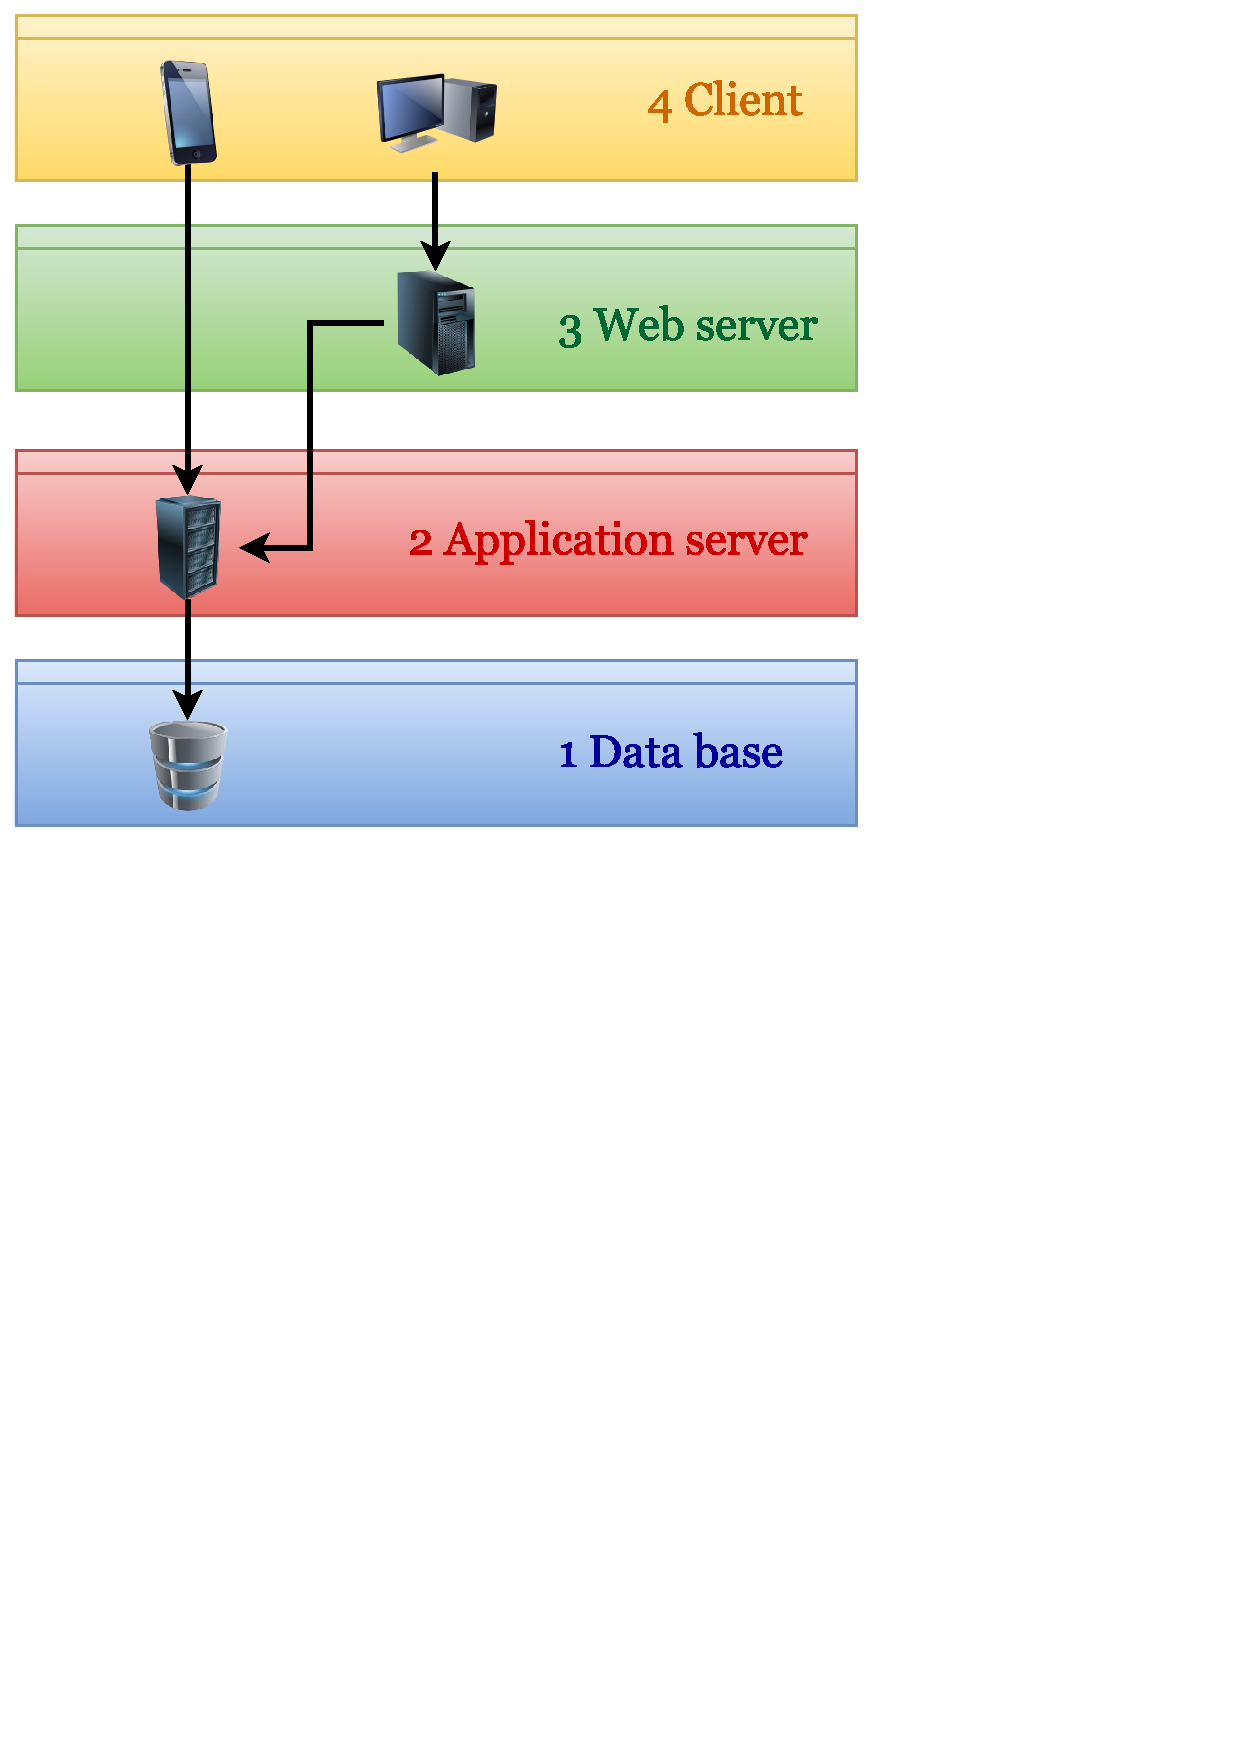
\includegraphics[width=0.7\textwidth]{diagrams/layers.pdf}
\caption{Layers of the system.}
\label{fig:layers}
\end{figure}

The interactions between the main components are shown in the figure \ref{fig:high_level_components} and are asynchronous, except for the interface between the application server and the database, which is synchronous.

\begin{figure}[h]
\centering
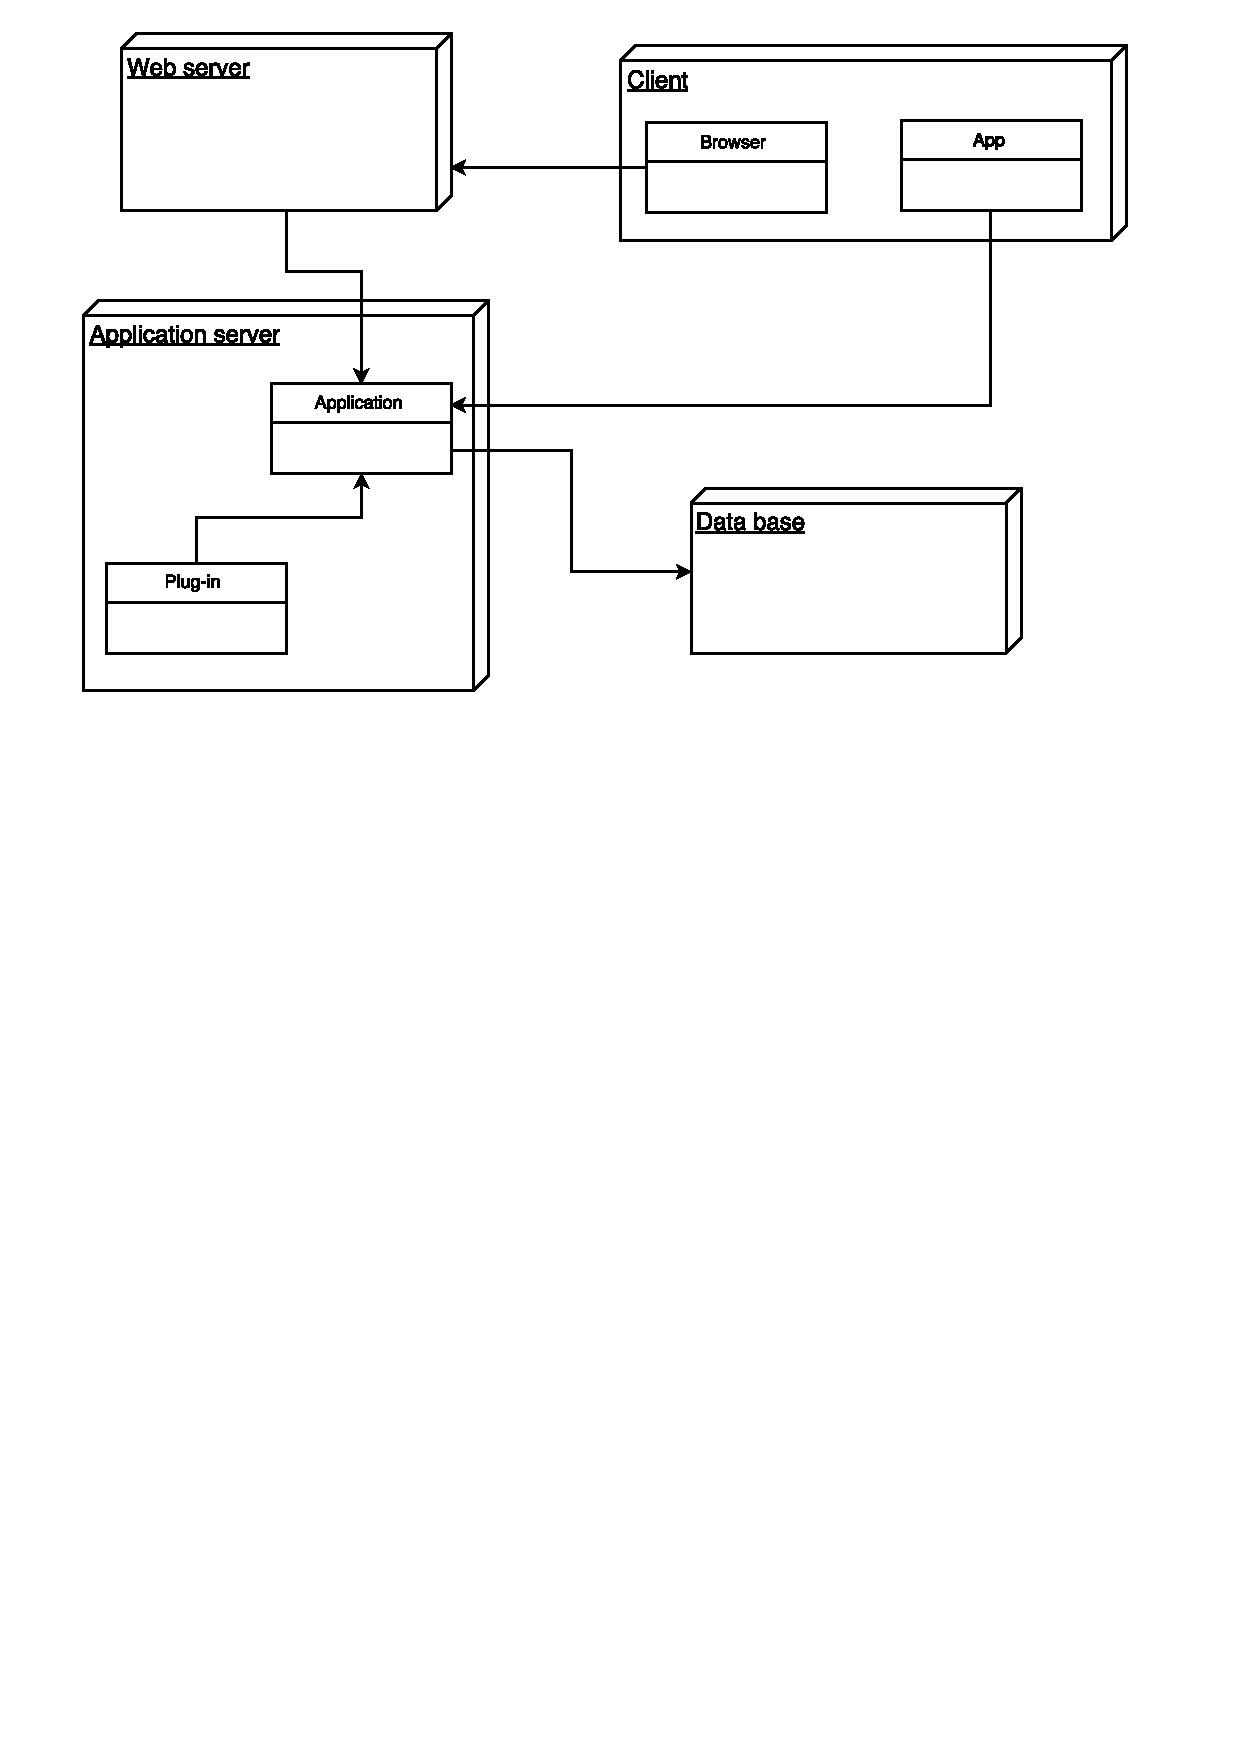
\includegraphics[width=\textwidth]{diagrams/high_level_components.pdf}
\caption{High level components of the system.}
\label{fig:high_level_components}
\end{figure}
